\documentclass[11pt]{article}

\usepackage[utf8]{inputenc}
\usepackage[english]{babel}
\usepackage{hyperref}

\usepackage[square,numbers]{natbib}
\bibliographystyle{plainnat}
\setcitestyle{authoryear,open={(},close={)}}

\usepackage{amsfonts, amsmath, amssymb, amsthm}

\newtheorem{theorem}{Theorem}[section]

\usepackage{graphicx}

\usepackage[margin=1in]{geometry}

\usepackage[utf8]{inputenc}
\usepackage{fancyhdr}
 
\pagestyle{fancy}
\fancyhf{}

\rhead{Benjamin Cox}
\chead{Statistical Consultancy -- Non-Assessed Problem}
\lhead{Due 17th October}
\rfoot{Page \thepage}

\begin{document}

\section{Introduction}
We consider data on the time taken for men and women to complete the 100, 200, and 400 metre dashes in the Olympics from 1900 to 2016 (it should be noted that data for the women's 100, 200, and 400 metre dash became available in 1928, 1948, and 1964 respectively). 

\section{Statistical Analysis}
We begin by transforming the data from times to speed using $s = d/t$. This gives us more easily interpreted data, as well as allowing for comparison between dashes. We now perform two linear regression analyses; one assuming that the rate of change of speed is the same for both men and women, and one making no such assumption.  \\

Table \ref{tab:reg1} shows the regression coefficients of the parallel regression, while Table \ref{tab:regmen} shows the regression for men only. Note that in both cases all parameters are highly significant, and that for the 100m the difference between men and women is about 1 metre per second in the parallel model. Table \ref{tab:regwom} contains the regression coefficients for the women's model.

The observations from these models line up for the 100m dash: the effect of the year is (almost) the same. The intercept is lower for women individually, but this is made up for by the slightly higher rate of increase applied over 1900 years. Overall these tables come to much the same conclusion: in the 100m dash men are faster than women by approximately 1 m/s, and both are getting faster on average by 1.07 m/s every 100 years.

\begin{table}[ht]
\centering
\begin{tabular}{rrrrr}
  \hline
 & Estimate & Std. Error & t value & Pr($>$$|$t$|$) \\ 
  \hline
(Intercept) & -11.1227 & 1.2604 & -8.82 & 0.0000 \\ 
  Year & 0.0107 & 0.0006 & 16.58 & 0.0000 \\ 
  SexWomen & -0.9499 & 0.0418 & -22.71 & 0.0000 \\ 
   \hline
\end{tabular}
\caption{Table of parallel regression coefficients for 100m}
\label{tab:reg1}
\end{table}

\begin{table}[ht]
\centering
\begin{tabular}{rrrrr}
  \hline
 & Estimate & Std. Error & t value & Pr($>$$|$t$|$) \\ 
  \hline
(Intercept) & -10.2911 & 1.3355 & -7.71 & 0.0000 \\ 
  Year & 0.0102 & 0.0007 & 15.03 & 0.0000 \\ 
   \hline
\end{tabular}
\caption{Table of regression coefficients for men's 100m}
\label{tab:regmen}
\end{table}

\begin{table}[ht]
\centering
\begin{tabular}{rrrrr}
  \hline
 & Estimate & Std. Error & t value & Pr($>$$|$t$|$) \\ 
  \hline
(Intercept) & -14.0452 & 2.6279 & -5.34 & 0.0000 \\ 
  Year & 0.0117 & 0.0013 & 8.76 & 0.0000 \\ 
   \hline
\end{tabular}
\caption{Table of regression coefficients for womens 100m}
\label{tab:regwom}
\end{table}

\pagebreak

Performing the same analysis for the 200m dash we obtain similar results: men are faster than women by approximately 1.05 m/s with both sexes increasing speeds by 1.12 m/s every 100 years.

When we look at the 400m dash things get a good deal more interesting. Tables \ref{tab:400b}, \ref{tab:400m}, and \ref{tab:400w} contain the regression coefficients for the 400m dash for parallel, men, and women respectively.

\begin{table}[ht]
\centering
\begin{tabular}{rrrrr}
  \hline
 & Estimate & Std. Error & t value & Pr($>$$|$t$|$) \\ 
  \hline
(Intercept) & -11.1839 & 1.4865 & -7.52 & 0.0000 \\ 
  Year & 0.0102 & 0.0008 & 13.42 & 0.0000 \\ 
  SexWomen & -1.0036 & 0.0530 & -18.95 & 0.0000 \\ 
   \hline
\end{tabular}
\caption{Table of regression coefficients for 400m}
\label{tab:400b}
\end{table}

\begin{table}[ht]
\centering
\begin{tabular}{rrrrr}
  \hline
 & Estimate & Std. Error & t value & Pr($>$$|$t$|$) \\ 
  \hline
(Intercept) & -12.0157 & 1.3964 & -8.60 & 0.0000 \\ 
  Year & 0.0106 & 0.0007 & 14.89 & 0.0000 \\ 
   \hline
\end{tabular}
\caption{Table of regression coefficients for men's 400m}
\label{tab:400m}
\end{table}

\begin{table}[ht]
\centering
\begin{tabular}{rrrrr}
  \hline
 & Estimate & Std. Error & t value & Pr($>$$|$t$|$) \\ 
  \hline
(Intercept) & -4.4243 & 5.4245 & -0.82 & 0.4306 \\ 
  Year & 0.0063 & 0.0027 & 2.30 & 0.0401 \\ 
   \hline
\end{tabular}
\caption{Table of regression coefficients for women's 400m}
\label{tab:400w}
\end{table}

Note that Table \ref{tab:400w} shows that women are increasing speed at approximately half the rate of men (given in Table \ref{tab:400m}). Overall the rate of increase is closer to that of men's, however that is due to the relative abundance of men's data compared to women's. This difference is clearly illustrated in Figure \ref{fig:npplots}. \\

Figure \ref{fig:npplots} actually gives us a good amount of information. The intervals indicated on the regression plots are the prediction intervals. We can see that they never overlap for the 100m and 200m dashes. This means that we can be reasonably confident that men will be faster than women in the period covered.

The intervals do overlap at the beginning of the time period for the 400m dash. This is more due to the lack of data on the women's 400m dash before 1964, which leads to the relative broadness of this interval.\\

Looking at both Figures \ref{fig:npplots} and \ref{fig:pplots} we see that it is reasonable to consider sex as a constant factor (i.e. a constant number subtracted or added depending on sex) for the 100m and 200m, but it is less reasonable for the 400m, as the slope for the women when considered individually is quite a bit shallower. 

Looking at our residual plots we see no pattern in the residuals when compared to the fitted. This means that we have not left out an obvious term in our model (i.e. seasonality). We could improve our model by adding term enforcing a theoretical upper limit, but this is beyond the scope of this analysis.



\section{Conclusions}

We conclude that in the Olympics men are faster than women overall. Both sexes are improving speeds at a good rate. This rate is similar for both men and women in the shorter distance races, although men are improving faster in the 400m race when compared to women.

We will also note that longer distance races have slower speeds than their short distance counterparts. This is to be expected, as endurance pays more of a role in these races than in short races.

\subsection{An addendum on proper statistical methods, and why transformations are important}

The \citet{oly2156} paper `Momentous sprint at the 2156 Olympics?', uses time as our regression variable, rather than speed. This has a few effects, one of which being that it is possible, in the future, for the model to predict a time of 0, or indeed a negative time. This non-physical behaviour is prevented by taking the transform from speed to distance. Eventually we will have people running faster than cars, and eventually the speed of light, but this could be prevented by adding an exponential term, giving an upper limit to human speed, but this would require more in depth analysis than the data we have allows. 

It is also easier to understand speed than time taken to cover distance, as well as making races of different distance immediately comparable. 

\bibliography{references}

\begin{figure}
 
  \centering
    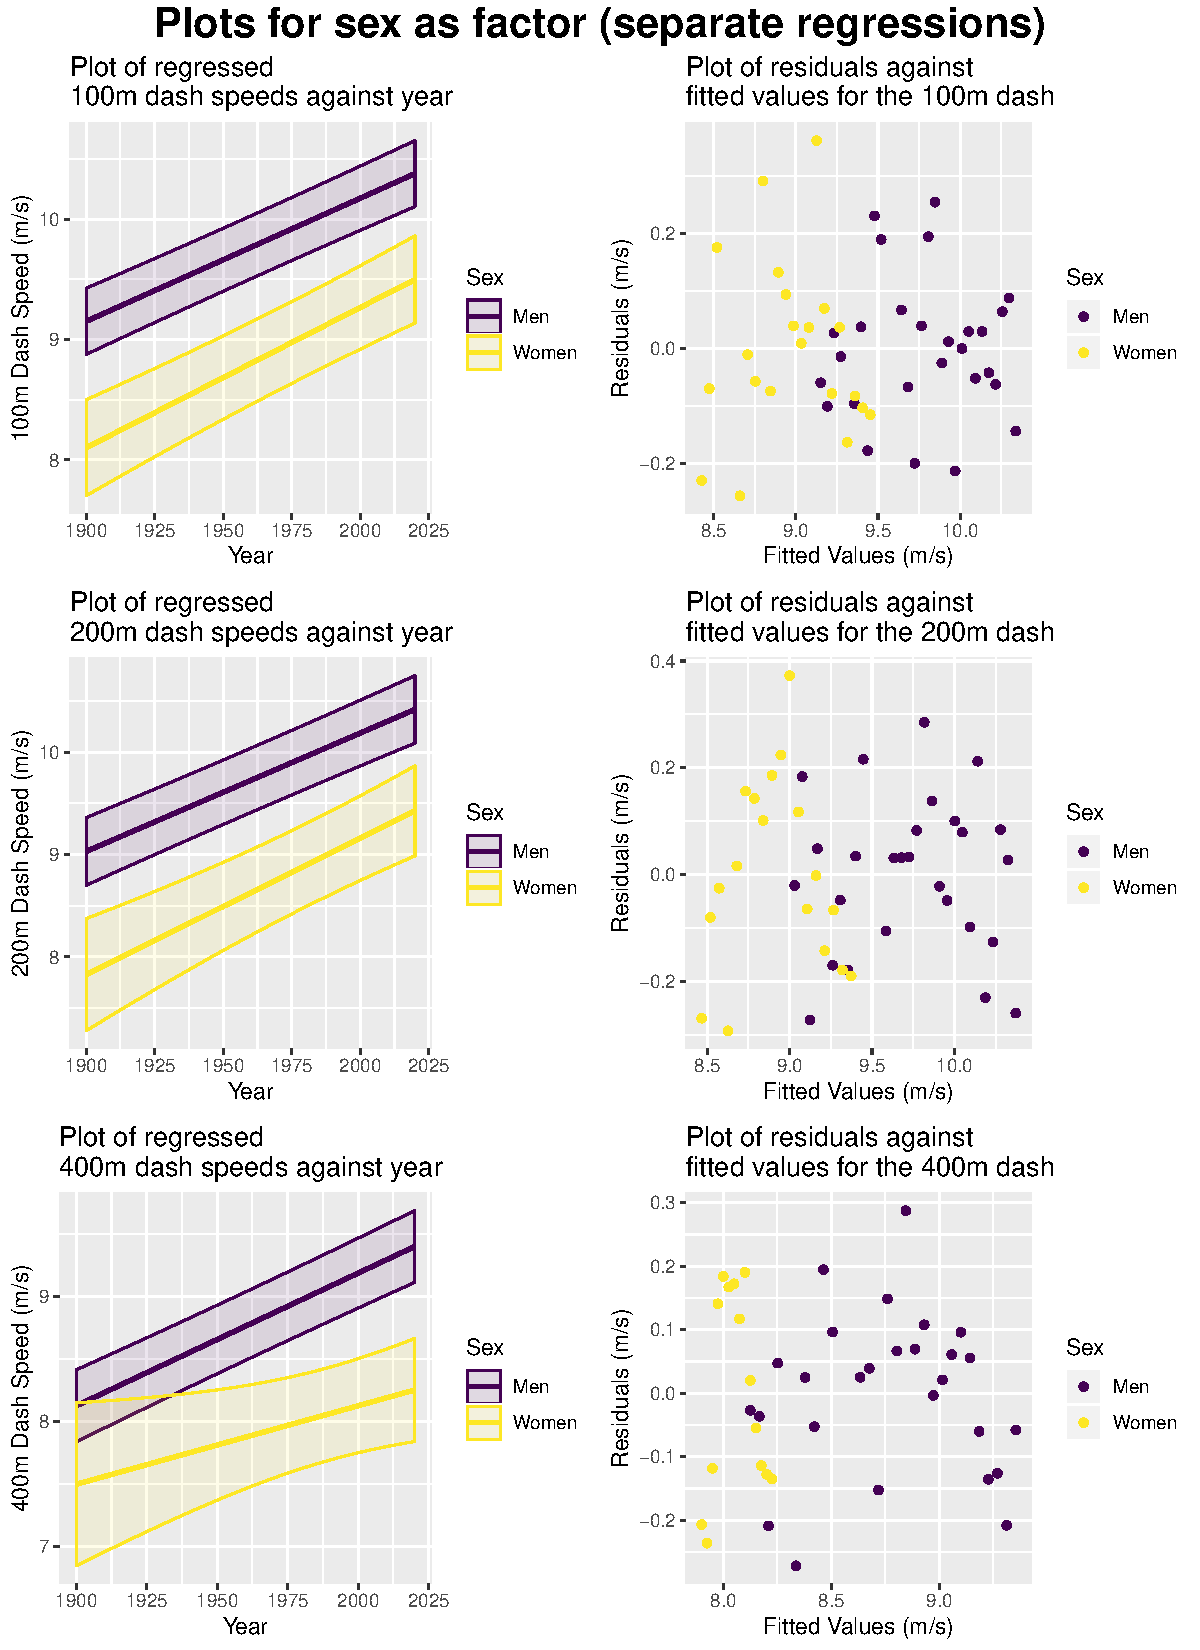
\includegraphics[width=\textwidth]{npplots}
 \caption{Plots showing properties of the separate regressions}
\label{fig:npplots}
\end{figure}

\begin{figure}
	
	\centering
	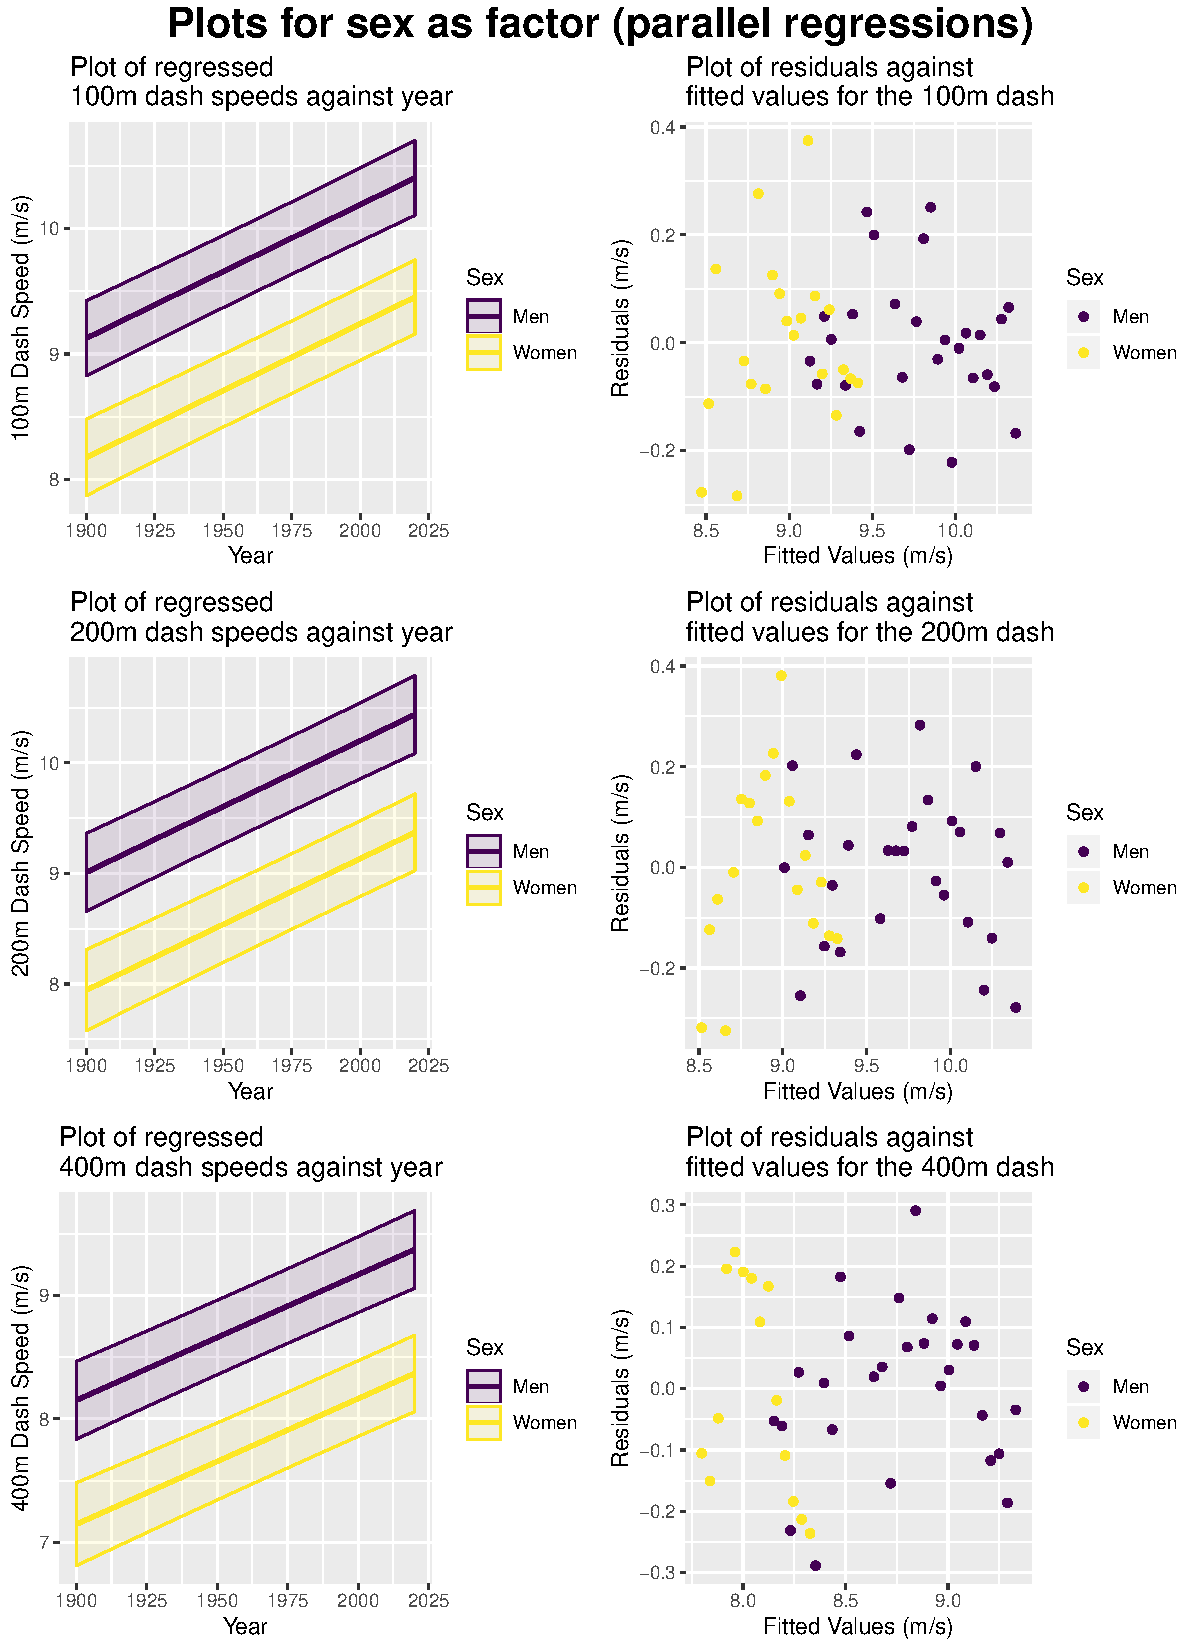
\includegraphics[width=\textwidth]{pplots}
	\caption{Plots showing properties of the parallel regressions}
	\label{fig:pplots}
\end{figure}

\end{document}